% !TEX root = ../main.tex
\chapter{Hva er fysikk?}
\intro{Verden består av så mye forskjellig. Her har vi natur, med skoger og fjell, elver og vann. Her lever alle mulige biologiske vesener. Her finner vi også mennesket, som bygger hus, skyskrapere og teknologiske dupeditter som mobiltelefoner. Der oppe på kuleskallet ser vi stjerner og kométer, supernovaer og nordlys. Felles for alle disse svært forskjellige delene av verden er at det lar seg beskrive av matematikk. Dette er jo på en måte helt spinnvilt. Pionerene innen vitenskap, slik som Johannes Kepler, som oppdaget at planetene går i ellipser, og Isaac Newton, som oppdaget at det finnes en kraft som trekker planetene mot solen, var nok ganske forbløffet over at de kunne finne ut av dette ved hjelp av matematikk. Som Galileo Galilei sa det:
\begin{center}
    \textit{``Philosophy is written in this grand book, the Universe. But the book cannot be understood unless one first learns to comprehend the language and interpret the characters in which it is written. It is written in the language of mathematics, and its characters are triangles, circles, and other geometrical figures, without which it is humanly impossible to understand a single word of it. Without these, one is wandering about in a dark labyrinth.''}\cite{galilei1957assayer}
\end{center}

\tanke{}{%
    Kan alt i verden beskrives i matematikk? Hva med \textit{kjærlighet} eller \textit{bevissthet}? Slike vanskelige, filosofiske spørsmål skal vi ikke vsare på i dette kompendiet, men de er verdt å merke seg.}

\paragraph{I dette kapitlet} introduserer vi begrepet \textit{fysiske størrelser}, ser på SI-enheter og enkle regler for enhetsregning, og går gjennom signifikante siffer og standardform.}

\spm{}{%
\item Hva er fysikk?
\item Hvordan beskriver vi virkeligheten med matematikk?}

\section{Hva er fysikk?}

Fysikken er vitenskapen som studerer naturen, helt fra det minste (beskrevet av kvantefysikk) og helt opp til universet som helhet (kosmologi). Fysikken kan deles i flere grupper, slik som mekanikk, termofysikk, bølgefysikk, fluidmekanikk, elektromagnetisme, kvantemekanikk, relativitetsteori osv. I TRES0312 blir det fokus på følgende områder:
\begin{itemize}
    \item Mekanikk
    \vspace{-0.75em}
    \item Fysikk i væsker og gasser
    \vspace{-0.75em}
    \item Termofysikk
    \vspace{-0.75em}
    \item Elektrisitetslære
\end{itemize}
Det er spesielt det første temaet; mekanikk, som blir lagt vekt på. Ca. halvparten av kurset går med til emner fra dette temaet.

\section{Fysiske størrelser}
Når vi anvender matematikk for å beskrive naturen, kommer vi frem til noe vi kan kalle \textit{fysiske størrelser}. La oss se litt på dette.

En fysisk størrelse har et tall knyttet til seg, men også en énhet. Ta forelesers vekt og høyde som eksempel. Vi kan tenke oss at foreleser veier $m=75\,\textrm{kg}$ og har en høyde på $h=1.75\,\textrm{m}$. Både \textit{vekt} og \textit{høyde} er fysiske størrelser, og vi gir gjerne disse størrelsene en variabel som navn (i dette tilfellet $m$ for masse og $h$ for høyde). Tallet i hver av disse fysiske størrelsene indikerer noe om \textit{mengde} eller \textit{omfang}. La oss kalle det \textit{verdi}.  Tallet sier noe om verdi.
Det er ikke tilstrekkelig å spesifisere verdien. For $m=75$ sier lite. 75 \textit{hva da}?? Vi må spesifiserer hva målestokken er. Dette kaller vi å spesifisere \textit{måleenhet}, også kalt bare \textit{enhet}. Alle objekter som har samme enhet kan sammenliknes. For eksempel kan jeg si at $h=1.74\,\textrm{m}$ er mindre enn høyden $H=1.84\,\textrm{m}$. Men jeg kan ikke si at $h=1.74\,\textrm{m}$ er mindre enn $m=75\,\textrm{kg}$. Hva i huleste skulle et slikt utsagn bety? Vi ser altså at i fysikken er både verdi og enhet viktig.

\defnr{Fysisk størrelse}{fys-storrelse}{En \textit{fysisk størrelse} har både \textit{verdi} og \textit{enhet}:
\begin{align*}
    &\textrm{Fysisk størrelse} = \textrm{verdi} \cdot \textrm{enhet}.
\end{align*}
}

\exm{Lengde}{%
Et enkelt eksempel er avstanden $L$ fra Oslo til Trondheim:
\[L = 500 \cdot \textrm{kilometer}\]
}

\tanke{}{Hvor mange forskjellige enheter trenger man for å beskrive \textit{alt} i naturen?}
I tabellen under ser vi noen av de mest sentrale fysiske størrelsene i mekanikk-delen av pensum, sammen med målenheten for disse størrelsene.
\begin{table}[H]
\centering
\renewcommand{\arraystretch}{1.3}
\begin{tabular}{|l|c|l|}
\hline
\rowcolor{blue!20!black!10}
\textbf{Fysisk størrelse} & \textbf{Enhet} & \textbf{Beskrivelse} \\
\hline
Tid & s & Hvor lenge noe varer \\
Lengde & m & Avstand mellom to punkter \\
Masse & kg & Hvor mye stoff det er i et objekt \\
Fart & m/s & Hvor raskt noe beveger seg \\
Akselerasjon & m/s$^2$ & Hvor raskt farten endrer seg \\
Kraft & N & Vekselvirkning mellom legemer \\
Energi & J & Potensiale for vekselvirkning.\\
\hline
\end{tabular}
\caption{Eksempler på fysiske størrelser og deres enheter.}
\end{table}
I det følgende skal vi se på et standardisert system for enheter, og hvordan vi kan regne med enheter.
\subsection{SI-enheter}
Man kunne jo tenkt at det trengs veldig mange enheter for å beskrive alt i naturen, ettersom naturen består av veldig mye forskjellig. Men det viser seg at man ikke trenger flere enn 7 forskjellige enheter. Det finnes mange forskjellige systemer for enheter. Felles for dem er at de koker ned til 7 unike enheter. I dette faget skal vi benytte SI-enheter, som er det internasjonale enhetssystemet sitt system, og benyttet i mange land. Figur \ref{fig:SI_enheter} viser en illustrasjon av SI-enhetene, og i dette faget skal vi benytte alle, så nær som \textit{candela}, som er måleenhet for \textit{opplevd lysstyrke}.

\begin{figure}[ht!]
\centering
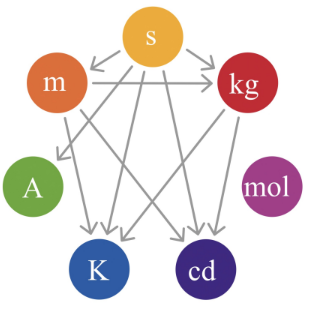
\includegraphics[width=0.3\textwidth]{Images/Kapittel1:introduksjon/SI-enheter.png}
\caption{SI-enhetene}
\label{fig:SI_enheter}
\end{figure}

Tabell~\ref{tab:SI_enheter} viser SI-enhetene og de naturkonstantene som bestemmer dem.

\begin{table}[H]
\caption{SI-enhetene og de naturkonstantene som definerer dem (2018-definisjonen). Fargede navn markerer de mest sentrale i dette kurset.}
\label{tab:SI_enheter}
\centering
\small
\renewcommand{\arraystretch}{1.3}
\begin{tabular}{|l|c|l||m{3.8cm}|c|m{3.6cm}|}
\hline
\rowcolor{blue!20!black!10}
\textbf{Måleenhet} & \textbf{Symbol} & \textbf{Fysisk størrelse} &
\textbf{Bestemt av (naturkonstant)} & \textbf{Symbol} & \textbf{Verdi (eksakt)} \\
\hline
Sekund    & s   & Tid             & Cesium-frekvens (hyperfin overgang)           & $\Delta\nu_{Cs}$ & $9\,192\,631\,770\ \text{Hz}$ \\
Meter     & m   & Avstand         & Lyshastigheten i vakuum                       & $c$              & $299\,792\,458\ \text{m/s}$ \\
Kilogram  & kg  & Masse           & Plancks konstant                              & $h$              & $6.626\,070\,15\cdot10^{-34}\ \text{J\,s}$ \\
Ampere    & A   & Elektrisk strøm & {\color{natKonstCol}Elementærladning}         & $e$              & $1.602\,176\,634\cdot10^{-19}\ \text{C}$ \\
Kelvin    & K   & Temperatur      & {\color{natKonstCol}Boltzmanns konstant}      & $k_B$            & $1.380\,649\cdot10^{-23}\ \text{J\,K}^{-1}$ \\
Mol       & mol & Stoffmengde     & {\color{natKonstCol}Avogadros konstant}       & $N_A$            & $6.022\,140\,76\cdot 10^{23}\ \text{mol}^{-1}$ \\
Candela   & cd  & Lys-intensitet  & Luminøs effektivitet                          & $K_{cd}$         & $683\ \text{lm\,W}^{-1}$ \\
\hline
\end{tabular}
\end{table}
I 2018 vedtok Generalkonferansen for mål og vekt at SI-systemet ikke lenger skal definires ut ifra menneskeskapte prototyper, slik som gullstandarden for 1\,kg i Paris og den slags. I stedet skal enhetene definieres ut ifra fysiske konstanter, som vist i høyre del av Tabell~\ref{tab:SI_enheter}. En skjematisk oppsummering av sammenhengen er gitt i Figur~\ref{fig:SI_enheter2}.

\begin{figure}[H]
    \centering

\includegraphics[width=0.5\linewidth]{Images/Kapittel1:introduksjon/SI-enheter2.png}
    \caption{Figuren viser hvilke fysiske konstanter som definerer de enkelte SI-enhetene. [Av Emilio Pisanty – Eget verk, CC BY-SA 4.0, https://commons.wikimedia.org/w/index.php?curid=50713156]}
\label{fig:SI_enheter2}
\end{figure}
Den ytterste ringen i Figur~\ref{fig:SI_enheter2} representerer de \textit{naturkonstantene} som er listet i høyre del av Tabell~\ref{tab:SI_enheter}. De med farget navn er mest sentrale i dette kurset.

\oppgaver{SI-enheter}{si-enheter}{%
Oppgi SI-enheten og enhetssymbolet for følgende fysiske størrelser:
\begin{enumerate}[a)]
    \item Masse
    \item Tid
    \item Temperatur
    \item Elektrisk strøm
    \item Lengde
\end{enumerate}
}

\subsection{Å regne med enheter}
Grunnen til at det ikke finnes mer enn 7 enheter er at det finnes lover mellom de forskjellige delene av fysikken som gjør at enkelte enheter kan skrives ved å bruke kombinasjoner av andre, mer fundamentale enheter. La oss ta \textit{fart} som eksempel.
\exm{Enhet for fart}{%
Når vi skal gi et variabel-navn til \textit{fart} bruker vi ofte bokstaven $v$ (forkortelse for det engelske \textit{velocity}). La oss si at faren til en bil er
\[v=50 \textrm{km}/\textrm{h}.\]
Her ser vi at enheten for fart, nemlig $\textrm{km}/\textrm{h}$ kan skrives ved hjelp av enhetene for strekning (km) og tid (h, for engelske \textit{hour}\footnote{Både $t$ for \textit{time} og  $h$ for \textit{hour} er mye brukte forkortelser. Du står derfor fritt til å velge selv hvilken forkortelse du vil benytte.}). Vi trenger altså ikke en egen enhet for fart.
}
Her har vi, uten å si det, brukt sammenhengen $v=s/t$ for å finne enhetene for farten $v$. Det faktum at det finnes sammenhenger og lover mellom forskjellige deler av fysikken, medfører at vi kan regne på enheter, slik som vi regner med tall. Da betrakter vi enhetene som algebraiske størrelser som kan legges sammen, ganges og deles på samme måte som tall. Det er viktig å huske at alle ledd i et uttrykk må ha samme enhet. Her er noen eksempler.

\exm{Sykkel på tog}{%
I forbindelse med en filminnspilling kjører Tom Cruise en motorsykkel ombord et cruisskip. Det er generelt en veldig dårlig idé. Men han gjør det likevel, og crus-skipet har en fart $v_\textrm{skip}=30\textrm{km}/\textrm{t}$. Tom har en fart $v_\textrm{T}=70\textrm{km}/\textrm{t}$ relativ til båten. Både Tom Cruise og cruisskipet kjører rett mot ei kai. Hvor stor fart har Tom i forhold til kaia?

\paragraph{Løsning:} For å finne ut dette kan vi legge sammen hastighetene.\\
% \vspace{6em}\\
% CHECK
Når begge objektene beveger seg i nøyaktig samme retning kan vi legge sammen størrelsene.
\begin{align*}
    30\textrm{km/t} + 70\textrm{km/t} = \underline{100 \textrm{ km/t}}
\end{align*}

}

\exm{Tilbakelagt avstand}{%
En dame på fjelltur går først 4 km mot nord og deretter 3 km mot vest. Hvor langt har hun gått totalt?\\

\paragraph{Løsning:}
% \vspace{6 em}\\
Pytagoras læresetning sier at i en rettinklet trekant er: \\
\begin{align*}
   \text{hypotenus} = \sqrt{\text{katet}^2 + \text{katet}^2}.
\end{align*}
4 km nord og 3 km vest gir derfor:
\begin{align*}
    \text{luftlinje} = \sqrt{(4\text{ km})^2 + (3\text{ km})^2} \text{k/m}= \sqrt{(4^2 + 3^2)\text{km}^2}=\sqrt{(4^2 + 3^2)}\text{ km}=\underline{5\text{ km}}
\end{align*}
}


\exm{Enhetsregning}{1) Regn ut hvor mange millimeter det er i 20 meter. \\

\paragraph{Løsning: } For å regne ut dette benytter vi en dekadisk omskriving av meter (mer om dette senere). Merk at \[1\,\textrm{m}= 10^3\,\textrm{mm}.\] Dermed har vi
\[20\textrm{m}=20\cdot 10^3\,\textrm{mm} = 20\,000\,\textrm{mm}.\]
}
Å kunne regne på enheter er en helt grunnleggende og veldig viktig egenskap når man holder på med fysikk. Det gir en god sjekk på om man har regnet riktig, og det hjelper en å se sammenhenger. 
\begin{myoppsum*}{Enhetsregning}
\begin{itemize}
    \item Man bruker algebra-regler for å regne med enheter.
    \item Alle ledd i et uttrykk må ha samme enhet
\end{itemize}
\end{myoppsum*}

\oppgave{Enhetsregning}{%
En bil kjører med fart $v = 90\,\textrm{km/t}$.
\begin{enumerate}[a)]
    \item Gjør om farten til m/s. \textit{Hint: } $1\,\textrm{km} = 10^3\,\textrm{m}$ og $1\,\textrm{t} = 3600\,\textrm{s}$.
    \item Kjøreturen varer i $t = 2.5\,\textrm{t}$. Finn tilbakelagt strekning i km og i m.
    \item Tyngdeakselerasjonen på månen er $g_\textrm{M} = 1.62\,\textrm{m/s}^2$. Gjør om til $\textrm{km/min}^2$.
\end{enumerate}
}

\subsection{Signifikante siffer}
Fysikk handler altså om å anvende matematikk på naturen. Dette kan vi gjøre fordi naturen er målbar. I fysikken er vi derfor helt avhengig av å \textit{måle}, altså å gjøre forsøk. Disse forsøkene gir aldri 100\% nøyaktige svar. Derfor er det viktig å ha kontroll på usikkerhet når man gjør fysikk. I dette kurset skal vi ikke se så mye på dette, men vi skal få med oss det mest grunnleggende, nemlig \textit{Signifikante siffer}. Signifikante siffer handler om å bruke riktig antall siffer i en utregning. La oss starte med å se på hvordan vi skal finne antall signifikante siffer. Tallet 459 har tre signifikante siffer, ettersom det består av tre siffer. Tallet 12\,001.\,03700 har 10 signifikante siffer, etter som det består av 10 siffer.
Men merk at tallet 0.00059400 kun har 5 signifikante siffer (nemlig 59400). Antall signifikante siffer telles nemlig fra \textit{første siffer som er forskjellig fra null.}

\begin{myoppsum*}{Signifikante siffer}
    \begin{itemize}
        \item Antall signifikante siffer regnes fra første tall forskjellig fra null.
        \item I en utregning skal svaret angis med samme nøyaktighet (antall siffer) som den \textit{minst nøyaktige} størrelsen som inngikk i beregningen.
    \end{itemize}
\end{myoppsum*}

\exm{Signifikante siffer}{%
Hvor mange signifikante siffer har tallene a) 165.00 b) 0.791400 og c) 14?

\paragraph{Løsning:}

\paragraph{a)} I dette tilfellet er første tall forskjellig fra null 1. Fra og med 1 er det 5 siffer. Det er derfor \doubleunderline{fem siffers signifikans.}

\paragraph{b)} Første tall forskjellig fra null er 7. Totalt er det \doubleunderline{6 siffers signifikans.}

\paragraph{c)} Her er det to siffer, så \doubleunderline{to siffers signifikans.}
}

\exm{Signifikante siffer i utregning}{Eline kjører 5.00 km på 6.0 minutter. Hvor fort kjører hun i gjennomsnitt?

\paragraph{Løsning: } Gjennomsnittsfart betegnes $\bar{v}$ og er rett og slett tilbakelagt strekning delt på tilbakelagt tid:
\[\bar{v}=\frac{5.00\textrm{km}}{6.0\textrm{min}}=0.83333...\textrm{km}/\textrm{min}=\doubleunderline{0.83\textrm{km}/\textrm{min}}\]
Dette kunne vi også gjort om til km$/$h ved å huske at $\textrm{min}=h/60.$ Dersom vi setter inn dette får vi

\[ \bar{v}=0.8333...\frac{\textrm{km}}{\textrm{h}/60}=60\cdot 0.8333...\,\textrm{km}/\textrm{h}=\doubleunderline{50\,\textrm{km}/\textrm{h}}\]
}

\begin{mymerk*}{Avrunding}
Vi minner om følgende regler for avrunding:
\begin{itemize}
    \item Tall fra 0-4 rundes ned. Tall fra og med 5 til 9 rundes opp.
    \item Avrunding til riktig antall signifikante siffer må skje helt tilslutt i en beregning! Derfor brukte vi 0.8333... i stedet for 0.83 da vi gjorde om fra km/min til km/h i eksemplet over. \textit{Bruk minst to ekstra siffer i utregningen!}
\end{itemize}
\end{mymerk*}

\oppgave{Signifikante siffer}{%
\begin{enumerate}[a)]
    \item Oppgi antall signifikante siffer i: $0.00420$, \ $3.14159$, \ $1\,200$ og $165.00$.
    \item Regn ut $12.3 \cdot 4.56$ og oppgi svaret med riktig antall signifikante siffer.
    \item Regn ut $18.0 / 4.5$ og oppgi svaret med riktig antall signifikante siffer.
\end{enumerate}
}

\subsection{Tall på standardform}
Standardform er en måte å skrive tall på som tydeliggjør både antall siffer og størrelsesorden. Et tall $T$ skrevet på standardform har følgende form:
\[
\label{eq:standardform}
\textrm{T}=t \cdot 10^n,
\]
hvor $t$ er et flyt-tall mellom 1 og 10. Eksemplet under tydeliggjør forhåpentligvis konseptet.

\exm{Standardform}{Skriv a) 0.07 b) 112 og c) 56\,700\,000 på standardform: \\

\paragraph{Løsning: }

\paragraph{a)} Tallet 0.07 har kun ett siffers signifikans. På standardform blir det da
\(7\cdot 10^{-2}\).

\paragraph{b)} Tallet 112 har tre siffers signifikans. På standardform får vi da
\(1.12\cdot 10^2\).

\paragraph{c)} Tallet 56\,700\,000 er et godt eksempel på et tall som er tvetydig slik det står. Tallet består av 8 siffer. Er dette et tall med 8 siffers signifikans, eller er det bare et veldig stort tall? Dersom tallet representerer antallet personer estimert i en folkemengde så er det nok ikke ment veldig nøyaktig. Dersom det representerer solgte varer i en butikk så er det nok helt nøyaktig, da butikken gjerne har et register over nøyaktig hvor mye som er solgt. I så tilfelle blir det \(5.6700000\cdot 10^7\) på standardform. Siden vi blir usikre, ringer vi rundt og får vite at dette tallet er et estimat på antall sandkorn i en sandhaug, og tallet har 2 siffers signifikans. Da er riktig skrivemåte
\[
5.7\cdot 10^7.
\]
Merk at vi her rundet opp fra 6 til 7, siden tallet til høyre for 6-tallet var større enn 4. Nå er både tallets nøyaktighet og størrelse lett å lese.
}

\oppgave{Standardform}{%
Skriv følgende tall på standardform:
\begin{enumerate}[a)]
    \item $0.000\,045$
    \item $3\,750\,000$
    \item $0.100$
    \item $299\,792\,458$
\end{enumerate}
Oppgi også antall signifikante siffer i hvert tall, slik du tolker det.
}

\subsection*{Dekadiske prefikser}
Å skrive tall på standardform er spesielt nyttig når tallene er veldig små eller veldig store. Da kan det også være nyttig å bruke såkalte \textit{dekadiske prefikser} som forkortelse for 10er-potensene. Tabell~\ref{tab:dekPref} oppsummerer disse.

\begin{table}[h!]
\centering
\renewcommand{\arraystretch}{1.2}
\begin{tabular}{|c|c|c|c|c|}
\hline
\rowcolor{blue!20!black!10}
$10^n$ & Prefiks & Symbol & Navn & Desimaltall \\
\hline
$10^{24}$ & yotta & Y & kvadrilion & 1 000 000 000 000 000 000 000 000 \\
$10^{21}$ & zetta & Z & trilliard  & 1 000 000 000 000 000 000 000 \\
$10^{18}$ & exa   & E & trillion   & 1 000 000 000 000 000 000 \\
$10^{15}$ & peta  & P & billiard   & 1 000 000 000 000 000 \\
$10^{12}$ & tera  & T & billion    & 1 000 000 000 000 \\
$10^{9}$  & giga  & G & milliard   & 1 000 000 000 \\
$10^{6}$  & mega  & M & million    & 1 000 000 \\
$10^{3}$  & kilo  & k & tusen      & 1 000 \\
$10^{2}$  & hekto & h & hundre     & 100 \\
$10^{1}$  & deka  & da& ti         & 10 \\
$10^{-1}$ & desi  & d & tidel      & 0.1 \\
$10^{-2}$ & centi & c & hundredel  & 0.01 \\
$10^{-3}$ & milli & m & tusendel   & 0.001 \\
$10^{-6}$ & mikro & $\mu$ & milliondel & 0.000001 \\
$10^{-9}$ & nano  & n & milliarddel  & 0.000000001 \\
$10^{-12}$& piko  & p & billiondel   & 0.000000000001 \\
$10^{-15}$& femto & f & billiarddel  & 0.000000000000001 \\
$10^{-18}$& atto  & a & trilliondel  & 0.000000000000000001 \\
$10^{-21}$& zepto & z & trilliarddel & 0.000000000000000000001 \\
$10^{-24}$& yocto & y & kvadrilliondel & 0.000000000000000000000001 \\
\hline
\end{tabular}
\caption{SI-prefikser for potenser av ti.}
\label{tab:dekPref}
\end{table}

\oppgave{Dekadiske prefikser}{%
\begin{enumerate}[a)]
    \item Et batteri har kapasitet $4\,200\,\textrm{mAh}$ (milliamperetimer). Skriv dette som et tall i Ah og på standardform.
    \item En avstand måles til $0.043\,\textrm{mm}$. Skriv dette i $\mu\textrm{m}$ (mikrometer) og i nm (nanometer).
    \item Lyset bruker ca. $499\,\textrm{s}$ fra solen til jorda. Lyset har fart $c = 3.00 \cdot 10^8\,\textrm{m/s}$. Finn avstanden fra solen til jorda i km og skriv svaret på standardform.
\end{enumerate}
}

\section{Flere oppgaver}

\oppgave{Fysisk størrelse}{%
Hva skal stå på venstre side av likhetstegnet?
\[
    \rule{4cm}{0.4pt} \;=\; \textrm{verdi} \cdot \textrm{enhet}
\]
}

\oppgave{Dekadiske prefikser -- matching}{%
Fyll inn faktoren for hvert prefiks i tabellen:
\begin{center}
\renewcommand{\arraystretch}{1.3}
\begin{tabular}{|l|c|c|}
\hline
\rowcolor{blue!20!black!10}
\textbf{Prefiks} & \textbf{Symbol} & \textbf{Faktor} \\
\hline
mega  & M & \\[4pt]
nano  & n & \\[4pt]
milli & m & \\[4pt]
centi & c & \\[4pt]
hekto & h & \\[4pt]
kilo  & k & \\[4pt]
giga  & G & \\[4pt]
\hline
\end{tabular}
\end{center}
}

\oppgave{Standardform}{%
Hvordan ser tallet $100.1$ ut når det er skrevet på standardform?
}

\oppgave{Signifikante siffer}{%
Per kjøper 1523 skruer til garasjen sin. Hver skrue veier $10.1\,\textrm{g}$.
Hvor mange signifikante sifre kan vi angi totalvekten til skruene med?
}
